\documentclass[10pt,a4paper]{article}
\usepackage[margin=1.7cm]{geometry}
\usepackage{times}
\usepackage{microtype}
\usepackage{graphicx}
\usepackage{booktabs}
\usepackage{url}
\usepackage{titlesec}
\usepackage{pgfplots}
\pgfplotsset{compat=1.18}
\usepackage[hidelinks]{hyperref}
\usepackage[numbers,sort&compress]{natbib}
\bibliographystyle{abbrvnat}

\setlength{\parskip}{1pt}
\setlength{\parindent}{0pt}
\titlespacing*{\section}{0pt}{4pt}{2pt}

% Per ISCB submission rules, the PDF must not contain title, authors,
% or affiliations -- those are collected via EasyChair.

\begin{document}

\begin{abstract}
\noindent
OntoClean \citep{Guarino2002OntoClean} provides a principled
methodology for detecting awkward taxonomic decisions in ontologies,
but its application requires manual annotation of every class with
five modal meta-properties, a cost that has kept it out of routine use
on biomedical ontologies. Here, we present a workflow that uses a
fine-tuned large language model to assign the meta-properties
automatically, an OWL reasoner to classify the hierarchy
\citep{Kazakov2014ELK}, and an OntoClean constraint checker over every
inferred (sub, super) pair. Applied to the Emotion Ontology (EMRO,
64~classes) the workflow surfaces 303~violations; an LLM auditor and a
manual review identify plausible modelling issues, including a
rigidity conflict on \texttt{sweat secretion}
$\sqsubseteq$ \texttt{secretion by tissue} and a contested unity
assignment on \emph{phenomenal cognitive experience}. The review also
exposes the central limitation: 83.5\% of the violations cascade from
a small number of upstream meta-property mislabelings on GO/BFO
process classes, where the model over-assigns identity to occurrents.
This limitation is reducible at zero training cost: re-running
inference with a BFO-grounded \citep{Arp2015BFO} system prompt drops
the violation count from 303 to 72 ($-76.2\%$), removes every R2
conflict, and collapses the residue to four specific class
mislabelings. LLM-assigned OntoClean is a viable -- if not yet
sufficient -- route to scaling principled ontology evaluation across
biomedicine.
\end{abstract}

\section{Introduction}
Biomedical ontologies such as the Gene Ontology
\citep{Ashburner2000GO} and the NCI Thesaurus encode the taxonomic
structure on which downstream annotation, semantic similarity, and
reasoning workflows depend. The internal coherence of that structure
matters: a single rigid kind placed under an anti-rigid superclass, or
a unity-bearing class under a parent that lacks unity, can propagate
silent errors through every dependent analysis. OntoClean
\citep{Guarino2002OntoClean} is the established methodology for
detecting such defects. It tags each class with five modal
meta-properties -- rigidity ($R$), identity ($I$), own-identity ($O$),
unity ($U$), dependence ($D$) -- and propagates inheritance constraints
(R1--R3, I1, U1--U2, O1) along the subsumption hierarchy.

In principle OntoClean should be a routine quality-assurance step for
bio-ontologies. In practice, the manual annotation of every class with
five modal meta-properties is prohibitive at the scale of GO, NCIt, or
even smaller ontologies that re-use them
\citep{Guarino2002OntoClean,Welty2001Supporting}. As a consequence,
OntoClean is rarely applied where it would be most informative -- on
biomedical ontologies that import upper terms from BFO
\citep{Arp2015BFO} and GO. Here, we present a workflow that uses a
fine-tuned large language model (LLM) to supply the meta-property
annotations automatically, and we ask two empirical questions on the
Emotion Ontology (EMRO) as a case study: does the workflow identify
real candidate modelling issues, and what are its current limitations?

\section{Methods}
We extract \texttt{(uri, label, definition, parent\_label)} for every
named class via OWLAPI~5.5.0. A LoRA-fine-tuned Qwen-2.5-7B-Instruct
\citep{Yang2024Qwen25} (\texttt{qwen7b-ontoclean}), trained on a
curated OntoClean dataset, predicts the five meta-properties and a
top-level classification (Sortal, Role, Mixin, Process, Quality,
\dots). We classify the asserted hierarchy with the ELK reasoner
\citep{Kazakov2014ELK} and check every inferred (sub, super) pair
against the OntoClean constraints R1--R3, I1, U1--U2 and the O1
warning. A second LLM pass then audits each violation row and emits a
verdict in \{\textsc{model\_error}, \textsc{cascades\_from\_direct},
\textsc{ontology\_issue}, \textsc{don't\_know}\}.

\textbf{Case study.} The Emotion Ontology
(EMRO,~\url{http://purl.bioontology.org/ontology/EMRO}, release
2026-03-30), 64~named classes, is small enough to permit manual audit
yet re-uses GO and BFO process terms as parents -- the regime where
OntoClean is most informative.

\textbf{Prompt-grounding experiment.} To characterise the workflow's
limits we re-ran inference with a BFO-augmented system prompt that
adds (i)~the continuant/occurrent distinction, (ii)~the rule that
occurrents default to $-I,-O,\sim\!U,+D$ unless an explicit identity
criterion is named, and (iii)~five worked examples (3 occurrents, 2
continuants). We did not update model parameters. We compared the two
runs by raw violation counts per constraint, by classification
distribution, and by row-level attribution to root mislabelings.

\section{Results}
\textbf{The workflow identifies candidate modelling issues.} On EMRO
the baseline run produces 303 violations across 370 (sub, super) pairs
(135 I1, 84 U1, 67 U2, 17 R2). The LLM auditor flags one row as a
genuine \textsc{ontology\_issue} -- the GO subsumption \texttt{sweat
secretion} $\sqsubseteq$ \texttt{secretion by tissue}, where the
asserted child sits under a non-rigid parent -- and two rows as
\textsc{don't\_know} on \emph{phenomenal cognitive experience}, a
class whose unity status is genuinely contested. Both findings are
useful flags for an EMRO maintainer.

\textbf{Aggregate counts overstate the defect rate.} The auditor
attributes the remaining 300 violations to 253
\textsc{cascades\_from\_direct} (83.5\% of all rows) and 47
\textsc{model\_error} rows that cluster on a single failure mode: the
LLM over-assigns $+I$ and $+U$ to GO/BFO process classes, although BFO
processes do not carry their own identity criteria. The classification
distribution mirrors this confusion, with 40/64 classes labelled Role
and 14/64 Mixin on what is in fact a process-heavy ontology. Aggregate
violation counts therefore conflate real modelling issues with
predictor cascades -- the central limitation of LLM-assigned OntoClean
as deployed today.

\textbf{A BFO-grounded prompt reduces cascades.} Re-running the same
model with the BFO-augmented prompt changes every one of the 64
predictions and reduces violation counts on every constraint
(Table~\ref{tab:headline}, Fig.~\ref{fig:violations}). The
classification distribution flips to a process-dominant reading
(53~Process, 7~Quality, 3~Sortal, 1~Mixin), and the entire R2 cluster,
including the \textsc{ontology\_issue} row, disappears. The 74
residual rows are not 74 independent errors: they trace to exactly
four root mislabelings, which together account for every row --
\texttt{system process} (44 rows: predicted $+I,+O,+U$ vs.\ true
$-I,-O,\sim\!U$), \texttt{regulation of biological quality} (12 rows;
predicted as Sortal), and \texttt{emotional experience} together with
\texttt{sensory experience} (12 + 6 rows; predicted as Sortals under a
$\sim\!U$ process chain).

\begin{table}[h]
\centering
\small
\caption{OntoClean violations on EMRO (64 classes) by constraint.}
\label{tab:headline}
\begin{tabular}{lrrr}
\toprule
Constraint & Baseline & BFO prompt & $\Delta$ \\
\midrule
I1 (identity not inherited)      & 135 & 27  & $-80.0\%$ \\
U1 (unity not inherited)         & 84  & 27  & $-67.9\%$ \\
U2 (anti-unity not inherited)    & 67  & 18  & $-73.1\%$ \\
R2 (rigid under non-rigid)       & 17  & \textbf{0} & $\mathbf{-100.0\%}$ \\
O1 (own-IC warning)              & --  & 2   & --      \\
\midrule
\textbf{Total violations}        & \textbf{303} & \textbf{72}  & $\mathbf{-76.2\%}$ \\
\bottomrule
\end{tabular}
\end{table}

\begin{figure}[h]
\centering
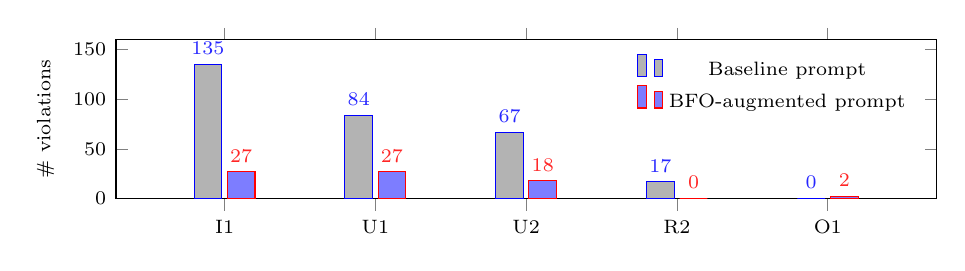
\begin{tikzpicture}
\begin{axis}[
    width=12cm, height=3.6cm,
    ybar=2pt, bar width=10pt,
    enlarge x limits=0.18,
    ymin=0, ymax=160,
    ylabel={\# violations},
    symbolic x coords={I1,U1,U2,R2,O1},
    xtick=data,
    nodes near coords,
    nodes near coords style={font=\scriptsize},
    legend style={at={(0.98,0.95)},anchor=north east,font=\scriptsize,draw=none},
    tick label style={font=\scriptsize},
    label style={font=\scriptsize},
    every axis plot/.append style={fill opacity=0.85,draw opacity=1},
]
\addplot+[fill=gray!70] coordinates {(I1,135) (U1,84) (U2,67) (R2,17) (O1,0)};
\addplot+[fill=blue!60] coordinates {(I1,27)  (U1,27) (U2,18) (R2,0)  (O1,2)};
\legend{Baseline prompt, BFO-augmented prompt}
\end{axis}
\end{tikzpicture}
\caption{OntoClean violations on EMRO before and after we augment the
system prompt with BFO upper-ontology guidance. We use the same
fine-tuned Qwen-2.5-7B model in both runs; only the system prompt
differs. Total: 303 $\rightarrow$ 72 ($-76.2\%$).}
\label{fig:violations}
\end{figure}

\section{Discussion}
LLM-assigned OntoClean is feasible as a scalable defect detector for
bio-ontologies: on EMRO it surfaces a small set of genuinely
interesting modelling questions -- a rigidity conflict on a GO
secretion subsumption and a contested unity assignment on phenomenal
experiences -- that a maintainer would want to review. However, the
same run also produces hundreds of cascading rows that look like
defects but trace back to predictor errors on upstream BFO/GO process
classes. This is the central practical limitation of the workflow:
without upper-ontology grounding, the LLM treats biomedical processes
as identity-bearing continuants and floods the report with spurious
cascades. The grounding experiment shows the limitation is not
fundamental: a five-sentence BFO occurrent rule with five worked
examples in the system prompt removes 76.2\% of violations and reduces
the residue to four specific mislabeled classes. Two of those four
(\emph{system process}, \emph{regulation of biological quality}) slip
past the rule because their definitions describe a capacity rather
than an event; the other two (\emph{emotional experience},
\emph{sensory experience}) reflect a long-standing philosophical
question about whether phenomenal experiences are substantial or
occurrent -- arguably a feature, not a defect, since this is exactly
the kind of decision OntoClean should surface.

\textbf{Limitations and future directions.} (1)~Aggregate violation
counts should not serve as quality signals without auditing, because
the predictor's cascades can dwarf real defects. (2)~Prompt
engineering with explicit BFO category rules is zero-cost and
deployable, but a permanent fix calls for fine-tuning data that
includes parent BFO categories as features. (3)~Generalisation beyond
EMRO remains to be shown; an experiment on a 300-class sample of the
NCI Thesaurus is in progress. (4)~The workflow still depends on a
human auditor to separate cascades from real defects; learning that
distinction directly is the natural next step.

\textbf{Reproducibility.} All inputs, predictions, violation files,
prompts and analysis scripts will be released under an open-source
licence on acceptance.

\textbf{Use of large language models.} In accordance with the ISCB
Acceptable Use of Large Language Models Policy, we disclose that LLMs
are the \emph{object of study} of this work: the fine-tuned
\texttt{qwen7b-ontoclean} predictor and the LLM auditor are research
artefacts, used as algorithmic techniques and as an evaluation aid in
the sense of the policy's acceptable uses (items 1 and 4). No LLM is
listed as an author. We did not supply confidential data to any model.
The text of this abstract was written by the authors.

\renewcommand{\refname}{\vspace{-0.4em}\normalsize References\vspace{-0.4em}}
\footnotesize
\begin{thebibliography}{9}
\setlength{\itemsep}{1pt}\setlength{\parsep}{0pt}
\bibitem{Guarino2002OntoClean}
N.~Guarino and C.~Welty.
\newblock Evaluating ontological decisions with OntoClean.
\newblock {\em Communications of the ACM}, 45(2):61--65, 2002.

\bibitem{Welty2001Supporting}
C.~Welty and N.~Guarino.
\newblock Supporting ontological analysis of taxonomic relationships.
\newblock {\em Data \& Knowledge Engineering}, 39(1):51--74, 2001.

\bibitem{Arp2015BFO}
R.~Arp, B.~Smith, and A.~D. Spear.
\newblock {\em Building Ontologies with Basic Formal Ontology}.
\newblock MIT Press, 2015.

\bibitem{Ashburner2000GO}
M.~Ashburner et al.
\newblock Gene Ontology: tool for the unification of biology.
\newblock {\em Nature Genetics}, 25(1):25--29, 2000.

\bibitem{Kazakov2014ELK}
Y.~Kazakov, M.~Kr\"otzsch, and F.~Simancik.
\newblock The incredible ELK: from polynomial procedures to efficient
  reasoning with ${\cal EL}$ ontologies.
\newblock {\em Journal of Automated Reasoning}, 53(1):1--61, 2014.

\bibitem{Yang2024Qwen25}
A.~Yang et al.
\newblock {Qwen2.5} technical report.
\newblock {\em arXiv:2412.15115}, 2024.
\end{thebibliography}

\end{document}
